% Provenance (never printed): see sources/outline_sources.md (Year 2: partial melting of the
% mantle; solidus and geotherm; decompression, hydration and heating; degree of melting;
% binary and ternary phase diagrams applied to rocks).
% Curves from figdata/bachelor-2/melting.py (Bowen 1915 diopside-anorthite, Bowen and
% Andersen 1914 forsterite-silica, Katz et al. 2003 melting of peridotite); exercise and
% problem values in the Book 4 scratch calculator calc/ch07.py.
\chapter{La fusión del manto}\label{ch:b2:mantle-melting}

El manto es sólido. Las ondas sísmicas de cizalla lo atraviesan de arriba abajo, y la
\omterm{def:b2:mantle-melting:peridotites}{peridotita} que sube de él es una roca cristalina. Sin embargo, solo a lo largo de las dorsales
oceánicas aporta unos veinte kilómetros cúbicos de corteza oceánica nueva cada año,
y cada metro cúbico de ella procede de un fundido. La paradoja se disuelve cuando se sabe
que el manto no se funde porque se calienta: se funde porque la
presión que soporta baja, o porque se le añade agua. Bajo una dorsal el
manto sube, su presión cae más deprisa que su temperatura, y cruza su
curva de fusión; sobre una placa que se hunde, el agua liberada por la placa rebaja esa
curva bajo la cuña del manto. En ambos casos solo se funde una pequeña fracción de la roca,
y esa fracción, separada de su residuo, se convierte en el basalto del
fondo oceánico y de los arcos volcánicos. Este capítulo describe primero la roca del
manto y los diagramas de fases que dicen cómo se funden esas rocas, y sigue después el
manto en su ascenso bajo una dorsal hasta el espesor de la corteza que forma.
% ledger: white:crust (Book 3), data:pb2002 (Book 3), katz03:solidus

\begin{recall}
\textbf{Del volumen de segundo año de los libros de química}: los diagramas de fases binarios, el
solidus y el liquidus, el punto eutéctico, la fusión congruente, las soluciones sólidas
y la regla de la palanca, según la cual las proporciones de dos fases coexistentes son
inversamente proporcionales a sus distancias a la composición global.
\textbf{De los libros de física}: el calor específico, el calor latente, la entropía
y el segundo principio, según el cual un proceso adiabático reversible conserva la entropía.
\textbf{Del volumen de primer año}: los principales minerales formadores de rocas, el olivino,
los piroxenos, el granate y la espinela, sus soluciones sólidas y el número de Mg; la
adiabata del manto, $\mathrm dT/\mathrm dz = \alpha gT/c_p$; la corteza oceánica, de
\qty[uncertainty-mode=separate]{7.1 \pm 0.8}{km} de espesor lejos de los puntos calientes y de
unos \qty{20}{km} sobre el núcleo de una pluma; las placas que subducen y el agua que
transportan. \textbf{Del \cref{ch:b2:elements-in-the-earth}}: el \omterm{def:b2:elements-in-the-earth:morb-oib}{basalto de dorsal oceánica}
(MORB), los coeficientes de reparto y los \omterm{def:b2:elements-in-the-earth:partition}{elementos incompatibles}.
\end{recall}

\section{La roca del manto}\label{sec:b2:mantle-melting:rock}

La roca del manto llega a la superficie como fragmentos arrastrados por los \omterm{def:b2:magma-emplacement:magma}{magmas}, los
xenolitos, y como la base de láminas de litosfera oceánica empujadas sobre los
continentes, las ofiolitas. Casi toda ella es \omterm{def:b2:mantle-melting:peridotites}{peridotita}.
% ledger: geo:peridotite (Book 2), tulane:ocean-basins (Book 2)

\begin{definition}[La peridotita y sus tipos]\label{def:b2:mantle-melting:peridotites}
Una \emph{peridotita}\index{peridotita} es una roca ultramáfica de grano grueso
que contiene más de un \qty{40}{\percent} de olivino, y el resto son piroxenos y un
poco de un mineral alumínico (espinela o granate). Una
\emph{dunita}\index{dunita} contiene más de un \qty{90}{\percent} de olivino. Por debajo
de ese valor, una \emph{lherzolita}\index{lherzolita} contiene ortopiroxeno y
clinopiroxeno; una \emph{harzburgita}\index{harzburgita} contiene ortopiroxeno pero
casi nada de clinopiroxeno; una wehrlita contiene clinopiroxeno pero casi nada de
ortopiroxeno. Las rocas con menos de un \qty{40}{\percent} de olivino son piroxenitas.
\end{definition}
% ledger: bgs:ultramafic

La clasificación se lee en un triángulo cuyos vértices son el olivino, el
ortopiroxeno y el clinopiroxeno (figura siguiente): cada punto representa una roca,
y sus distancias a los tres lados dan las proporciones de los tres
minerales. Una composición modelo del manto superior empobrecido que se funde bajo
las dorsales tiene un \qty{57}{\percent} de olivino,
un \qty{28}{\percent} de ortopiroxeno, un \qty{13}{\percent} de clinopiroxeno y un
\qty{2}{\percent} de espinela: una \omterm{def:b2:mantle-melting:peridotites}{lherzolita}.
% ledger: liang21:dmm-mode

\begin{omfigure}
\centering
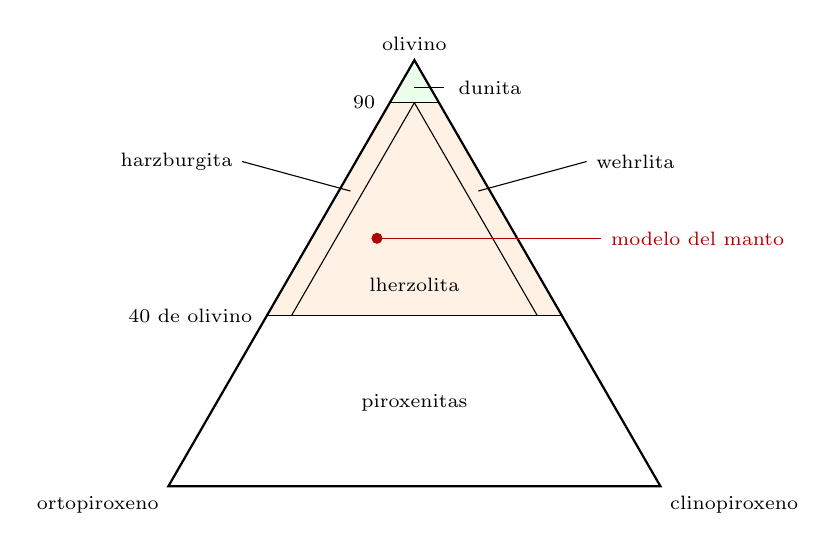
\begin{tikzpicture}[x=1.25cm, y=1.25cm, font=\scriptsize]
\coordinate (O) at (2.5,4.330); \coordinate (P) at (0,0); \coordinate (C) at (5,0);
\fill[green!8] (2.25,3.897) -- (2.75,3.897) -- (O) -- cycle;
\fill[orange!10] (1,1.732) -- (2.25,3.897) -- (2.75,3.897) -- (4,1.732) -- cycle;
\draw[thick] (O) -- (P) -- (C) -- cycle;
\draw (2.25,3.897) -- (2.75,3.897);
\draw (1,1.732) -- (4,1.732);
\draw (2.5,3.897) -- (1.25,1.732);
\draw (2.5,3.897) -- (3.75,1.732);
\node[anchor=south] at (O) {olivino};
\node[anchor=north east] at (P) {ortopiroxeno};
\node[anchor=north west] at (C) {clinopiroxeno};
\node[anchor=west] at (2.85,4.05) {dunita};
\draw (2.5,4.05) -- (2.8,4.05);
\node at (2.5,2.05) {lherzolita};
\draw (1.85,3.0) -- (0.75,3.3) node[anchor=east] {harzburgita};
\draw (3.15,3.0) -- (4.25,3.3) node[anchor=west] {wehrlita};
\node at (2.5,0.85) {piroxenitas};
\node[anchor=east] at (0.95,1.732) {\qty{40}{\percent} de olivino};
\node[anchor=east] at (2.2,3.897) {\qty{90}{\percent}};
\fill[red!70!black] (2.12,2.52) circle (2pt);
\draw[red!70!black] (2.12,2.52) -- (4.4,2.52) node[anchor=west] {modelo del manto};
\end{tikzpicture}
\par\smallskip{\small Clasificación de las \omterm{def:b2:mantle-melting:peridotites}{peridotitas} y las piroxenitas según sus
proporciones de olivino, ortopiroxeno y clinopiroxeno (según el esquema del British
Geological Survey). Las estrechas franjas a lo largo de los dos lados superiores contienen las
rocas casi sin clinopiroxeno (\omterm{def:b2:mantle-melting:peridotites}{harzburgita}) o sin ortopiroxeno (wehrlita).
El punto rojo es el manto superior modelo bajo las dorsales (57, 28 y
\qty{13}{\percent}, renormalizado sin su \qty{2}{\percent} de espinela).}
\end{omfigure}
% ledger: bgs:ultramafic, liang21:dmm-mode

Las tres \omterm{def:b2:mantle-melting:peridotites}{peridotitas} no son tres tipos de roca independientes: son etapas de
un mismo proceso. El clinopiroxeno y el mineral alumínico se agotan primero cuando
la \omterm{def:b2:mantle-melting:peridotites}{peridotita} se funde (\cref{sec:b2:mantle-melting:decompression}), de modo que una \omterm{def:b2:mantle-melting:peridotites}{lherzolita}
que ha perdido un fundido se empobrece en ellos; tras una fusión suficiente es una
\omterm{def:b2:mantle-melting:peridotites}{harzburgita}, y una roca que ha perdido casi todo su piroxeno es una \omterm{def:b2:mantle-melting:peridotites}{dunita}.
% ledger: katz03:melting

\begin{definition}[Manto fértil y manto residual]\label{def:b2:mantle-melting:fertility}
Un \emph{manto fértil}\index{manto fértil} es una \omterm{def:b2:mantle-melting:peridotites}{peridotita}, típicamente una
\omterm{def:b2:mantle-melting:peridotites}{lherzolita}, que aún contiene el clinopiroxeno y el mineral alumínico a partir de los
cuales se forma el basalto. Un \emph{manto residual}\index{manto residual} es la
\omterm{def:b2:mantle-melting:peridotites}{peridotita} que queda una vez extraído de ella un fundido: más pobre en
clinopiroxeno, aluminio, calcio y \omterm{def:b2:elements-in-the-earth:partition}{elementos incompatibles}, más rica en
olivino y con un número de Mg más alto.
\end{definition}

El \omterm{def:b2:isotope-geochemistry:reservoirs}{manto empobrecido} isotópico del \cref{ch:b2:isotope-geochemistry} es un reservorio,
definido por sus razones; un \omterm{def:b2:mantle-melting:fertility}{manto residual} es una roca, definida por lo que ha perdido.
Ambos están relacionados, ya que el \omterm{def:b2:isotope-geochemistry:reservoirs}{manto empobrecido} lo está porque se le extrajo
fundido hace mucho tiempo, pero uno se lee en un espectrómetro de masas y el otro
al microscopio.

\section{Diagramas de fases de las rocas}\label{sec:b2:mantle-melting:diagrams}

Una roca es una mezcla de minerales, y se funde en un intervalo de temperaturas, no en
un punto. Los diagramas que describen esto se midieron primero en mezclas de
minerales sintéticos puros, manteniendo una pequeña carga a una temperatura conocida hasta que
alcanzaba el equilibrio, templándola y buscando al microscopio vidrio,
que había sido líquido, y cristales.

\subsection*{Un eutéctico binario: diópsido y anortita}

Un basalto consta esencialmente de una plagioclasa cálcica y de un clinopiroxeno, y
Bowen eligió la anortita y el diópsido puros como su modelo más sencillo. Mezclados y calentados,
forman un sistema
eutéctico ordinario (figura siguiente): el diópsido funde a \qty{1391.5}{\celsius} y la anortita
a \qty{1550}{\celsius}, pero una mezcla de un \qty{58}{\percent} de diópsido y un
\qty{42}{\percent} de anortita en masa funde por completo a \qty{1270}{\celsius}.
% ledger: bowen15:di-an

\begin{omfigure}
\centering
\begin{tikzpicture}
\begin{axis}[omrecord, width=0.78\linewidth, height=6cm,
  xmin=0, xmax=100, ymin=1200, ymax=1600,
  xlabel={anortita (\unit{\percent} en masa)}, ylabel={temperatura (\unit{\celsius})},
  y tick label style={/pgf/number format/1000 sep={}},
  tick label style={font=\scriptsize}, label style={font=\small}]
\addplot[very thick, black] table[x=x_an, y=T] {figdata/out/bachelor-2-melting-di-an-liq.dat};
\addplot[only marks, mark=*, mark size=1.6pt, blue!70!black] table[x=x_an, y=T] {figdata/out/bachelor-2-melting-di-an-data.dat};
\draw[thick] (axis cs:0,1270) -- (axis cs:100,1270);
\draw[densely dotted, red!70!black, thick] (axis cs:20,1590) -- (axis cs:20,1270);
\draw[->, red!70!black, thick] (axis cs:20,1350) -- (axis cs:41,1272);
\fill[red!70!black] (axis cs:20,1350) circle (1.6pt);
\node[font=\scriptsize] at (axis cs:55,1500) {líquido};
\node[font=\scriptsize, align=center] at (axis cs:10,1300) {diópsido\\+ líquido};
\node[font=\scriptsize, align=center] at (axis cs:72,1360) {anortita + líquido};
\node[font=\scriptsize] at (axis cs:68,1235) {diópsido + anortita};
\node[font=\scriptsize, anchor=north east] at (axis cs:41,1267) {E, \qty{1270}{\celsius}};
\node[font=\scriptsize, anchor=west, red!70!black] at (axis cs:21,1360) {primer diópsido};
\end{axis}
\end{tikzpicture}
\par\smallskip{\small El sistema diópsido--anortita a la presión atmosférica, según
los experimentos de temple de Bowen (1915): temperaturas del liquidus (puntos, centros de
los intervalos de temple) y el eutéctico E. En rojo, el enfriamiento de un líquido con un
\qty{20}{\percent} de anortita: el diópsido cristaliza desde \qty{1350}{\celsius}, el
líquido desciende por el liquidus hasta E, y el resto cristaliza allí como una mezcla de
ambos minerales.}
\end{omfigure}
% ledger: bowen15:di-an

Leído desde arriba, el diagrama da el orden de cristalización. Un líquido con un
\qty{20}{\percent} de anortita empieza a cristalizar diópsido a
\qty{1350}{\celsius}; el líquido, al perder diópsido, se enriquece en anortita y
desciende por el liquidus hasta alcanzar el eutéctico, donde la anortita se une al
diópsido y la temperatura se mantiene en \qty{1270}{\celsius} hasta que se agota todo el
líquido. Leído desde abajo, dice cómo se funde la roca: sean cuales sean las proporciones de
los dos minerales, el primer líquido aparece a \qty{1270}{\celsius} y tiene la
composición eutéctica. Es la primera lección para el manto. El primer fundido de una
roca no tiene la composición de la roca: tiene la composición que fijan los
minerales a partir de los que se funde, y aparece a una temperatura muy inferior a los puntos de
fusión de todos ellos.

\subsection*{Fusión incongruente: forsterita y sílice}

Algunos minerales no funden en un líquido de su propia composición.

\begin{definition}[Fusión incongruente, punto peritéctico]\label{def:b2:mantle-melting:peritectic}
Un mineral presenta \emph{fusión incongruente}\index{fusión incongruente} cuando, al
calentarse, se descompone en otro sólido y un líquido de composición
distinta, en lugar de fundir en un líquido de su propia composición. En un diagrama de fases
binario, el punto en el que ese líquido coexiste con ambos sólidos es un
\emph{punto peritéctico}\index{punto peritéctico}: a diferencia de un eutéctico, no está
entre las composiciones de los dos sólidos.
\end{definition}

La enstatita, el ortopiroxeno magnésico \ce{MgSiO3}, funde de forma incongruente. A
la presión atmosférica se descompone a \qty{1557}{\celsius} en forsterita,
\ce{Mg2SiO4}, y un líquido algo más rico en sílice que ella misma; solo a
\qty{1577}{\celsius} se ha disuelto toda la forsterita (figura siguiente). Bowen
y Andersen hallaron en 1914 que la descomposición da un \qty{5.5}{\percent} de
forsterita y un \qty{94.5}{\percent} de líquido, como predice la regla de la palanca a partir de
las tres composiciones (\cref{exo:b2:mantle-melting:6}). Más hacia la sílice, la enstatita y la
cristobalita funden juntas en un eutéctico, a \qty{1543}{\celsius}.
% ledger: bowen14:mgo-sio2

\begin{omfigure}
\centering
\begin{tikzpicture}
\begin{axis}[omrecord, width=0.78\linewidth, height=6cm,
  xmin=40, xmax=66, ymin=1450, ymax=1950,
  xlabel={\ce{SiO2} (\unit{\percent} en masa)}, ylabel={temperatura (\unit{\celsius})},
  y tick label style={/pgf/number format/1000 sep={}},
  tick label style={font=\scriptsize}, label style={font=\small}]
\addplot[very thick, black] table[x=x_sio2, y=T] {figdata/out/bachelor-2-melting-fo-sio2-liq.dat};
\addplot[very thick, black, dashed] table[x=x_sio2, y=T] {figdata/out/bachelor-2-melting-fo-sio2-fo.dat};
\draw[thick] (axis cs:42.71,1450) -- (axis cs:42.71,1890);
\draw[thick] (axis cs:42.71,1557) -- (axis cs:60.86,1557);
\draw[thick] (axis cs:59.85,1450) -- (axis cs:59.85,1557);
\draw[thick] (axis cs:59.85,1543) -- (axis cs:66,1543);
\fill (axis cs:60.86,1557) circle (1.6pt);
\fill (axis cs:64.87,1543) circle (1.6pt);
\fill (axis cs:42.71,1890) circle (1.6pt);
\node[font=\scriptsize, anchor=south west] at (axis cs:42.9,1890) {la forsterita funde, \qty{1890}{\celsius}};
\node[font=\scriptsize] at (axis cs:56,1800) {líquido};
\node[font=\scriptsize] at (axis cs:48,1680) {forsterita + líquido};
\node[font=\scriptsize] at (axis cs:51,1500) {forsterita + enstatita};
\node[font=\scriptsize, align=center] at (axis cs:63,1495) {enstatita +\\cristobalita};
\node[font=\scriptsize, anchor=south] at (axis cs:61.3,1560) {P};
\node[font=\scriptsize, anchor=south] at (axis cs:64.87,1546) {E};
\node[font=\scriptsize, anchor=north, rotate=90] at (axis cs:42.71,1650) {\ce{Mg2SiO4}};
\node[font=\scriptsize, anchor=south, rotate=90] at (axis cs:59.85,1510) {\ce{MgSiO3}};
\end{axis}
\end{tikzpicture}
\par\smallskip{\small Parte del sistema \ce{MgO}--\ce{SiO2} a la presión
atmosférica, según Bowen y Andersen (1914). La enstatita (\ce{MgSiO3}) funde de forma
incongruente en el peritéctico P, a \qty{1557}{\celsius}, en forsterita y un
líquido con un \qty{60.9}{\percent} de \ce{SiO2}; E es el eutéctico enstatita--cristobalita,
a \qty{1543}{\celsius}. El liquidus de la forsterita solo se ha medido cerca de la
enstatita: la parte discontinua se traza recta hasta el punto de fusión de la forsterita.}
\end{omfigure}
% ledger: bowen14:mgo-sio2

El peritéctico es la segunda lección para el manto. Cuando una \omterm{def:b2:mantle-melting:peridotites}{peridotita} se funde, su
ortopiroxeno no se disuelve sin más: cede olivino al residuo y sílice
al fundido. El fundido es por tanto más rico en sílice que los piroxenos, y el
residuo más rico en olivino que la roca: el camino de la \omterm{def:b2:mantle-melting:peridotites}{lherzolita} a la \omterm{def:b2:mantle-melting:peridotites}{harzburgita}
y la \omterm{def:b2:mantle-melting:peridotites}{dunita}.

\subsection*{Tres componentes: el diagrama ternario}

Las rocas reales tienen más de dos minerales. Con tres, la composición necesita un
triángulo, y la temperatura se convierte en una tercera dimensión.

\begin{definition}[Diagrama de fases ternario, línea cotéctica, eutéctico ternario]\label{def:b2:mantle-melting:ternary}
Un \emph{diagrama de fases ternario}\index{diagrama de fases ternario} representa los
equilibrios de un sistema de tres componentes a una presión dada: cada punto de un
triángulo representa una composición, los vértices los componentes puros, y la
superficie del liquidus se dibuja como curvas de nivel de la temperatura o como los campos de los
minerales que cristalizan primero. Una \emph{línea cotéctica}\index{línea cotéctica} es
la línea a lo largo de la cual el líquido está saturado en dos minerales a la vez y
cristaliza ambos al enfriarse. Las líneas cotécticas descienden desde los eutécticos
binarios de los lados del triángulo y se encuentran en el \emph{eutéctico
ternario}\index{eutéctico ternario}, la temperatura más baja a la que existe líquido,
donde los tres minerales cristalizan juntos.
\end{definition}

\begin{method}[Leer una trayectoria de cristalización en un diagrama ternario]\label{met:b2:mantle-melting:ternary}
Sitúese la composición global $X$ en el triángulo y el campo en el que se encuentra:
el mineral de ese campo cristaliza primero. Mientras ese mineral cristaliza solo,
el líquido se desplaza en línea recta alejándose directamente del vértice del mineral,
a través de $X$, porque retirar un componente puro solo cambia su proporción; según la
regla de la palanca, la fracción másica de cristales es la distancia de $X$ al líquido
dividida por la distancia del vértice al líquido. Cuando el líquido alcanza una
\omterm{def:b2:mantle-melting:ternary}{línea cotéctica}, se une el segundo mineral y el líquido sigue la cotéctica
pendiente abajo hasta el \omterm{def:b2:mantle-melting:ternary}{eutéctico ternario}, donde cristaliza el último líquido. Un componente
que no entra en ninguno de los cristales permanece en el líquido, de modo que su concentración da
la fracción de líquido restante: $f_{\text{líquido}} = c_X/c_{\text{líquido}}$.
\end{method}

\begin{omfigure}
\centering
\begin{tikzpicture}[x=1cm, y=1cm, font=\scriptsize]
\coordinate (A) at (3,5.196); \coordinate (B) at (0,0); \coordinate (C) at (6,0);
\coordinate (eAB) at (1.2,2.078); \coordinate (eAC) at (4.65,2.338);
\coordinate (eBC) at (3.9,0); \coordinate (E) at (3.45,1.299);
\coordinate (X) at (3.0,3.118); \coordinate (L) at (3.0,1.455);
\fill[green!8] (A) -- (eAB) -- (E) -- (eAC) -- cycle;
\fill[orange!10] (B) -- (eAB) -- (E) -- (eBC) -- cycle;
\fill[blue!7] (C) -- (eAC) -- (E) -- (eBC) -- cycle;
\draw[thick] (A) -- (B) -- (C) -- cycle;
\draw[very thick, -{Stealth[length=4pt]}] (eAB) -- ($(eAB)!0.55!(E)$);
\draw[very thick] ($(eAB)!0.5!(E)$) -- (E);
\draw[very thick, -{Stealth[length=4pt]}] (eAC) -- ($(eAC)!0.55!(E)$);
\draw[very thick] ($(eAC)!0.5!(E)$) -- (E);
\draw[very thick, -{Stealth[length=4pt]}] (eBC) -- ($(eBC)!0.55!(E)$);
\draw[very thick] ($(eBC)!0.5!(E)$) -- (E);
\draw[red!70!black, thick, dashed] (A) -- (X);
\draw[red!70!black, very thick, -{Stealth[length=4pt]}] (X) -- (L);
\draw[red!70!black, very thick, -{Stealth[length=4pt]}] (L) -- ($(L)!0.85!(E)$);
\fill[red!70!black] (X) circle (2pt); \fill[red!70!black] (L) circle (1.6pt);
\fill (E) circle (2pt);
\node[anchor=south] at (A) {A}; \node[anchor=north east] at (B) {B};
\node[anchor=north west] at (C) {C};
\node[anchor=west, red!70!black] at (3.1,3.2) {$X$};
\node[anchor=north east, red!70!black] at (2.95,1.42) {$L_1$};
\node[anchor=north west] at (3.5,1.25) {E};
\node[anchor=east] at (eAB) {$e_{AB}$}; \node[anchor=west] at (eAC) {$e_{AC}$};
\node[anchor=north] at (eBC) {$e_{BC}$};
\node at (2.35,2.75) {campo de A}; \node at (1.55,0.7) {campo de B}; \node at (4.9,0.7) {campo de C};
\end{tikzpicture}
\par\smallskip{\small Un sistema \omterm{def:b2:mantle-melting:ternary}{eutéctico ternario} (esquema). Cada campo contiene
los líquidos de los que su mineral cristaliza primero; las \omterm{def:b2:mantle-melting:ternary}{líneas cotécticas} (flechas
hacia las temperaturas decrecientes) van de los eutécticos binarios $e$ al \omterm{def:b2:mantle-melting:ternary}{eutéctico
ternario} E. Un líquido $X$ del campo de A cristaliza A, y se aleja del vértice A
hasta encontrar la cotéctica A--B en $L_1$; A y B cristalizan entonces
juntos hasta E, donde se les une C (\cref{exo:b2:mantle-melting:11}).}
\end{omfigure}

Los sistemas de tres minerales formadores de rocas se leen del mismo modo. Las reglas que fijan cuántas fases pueden coexistir,
y las superficies de energía libre a partir de las cuales se calculan estos diagramas, corresponden al
volumen de tercer año de esta serie.

\section{Solidus, adiabata y tres maneras de fundir}\label{sec:b2:mantle-melting:solidus}

La \omterm{def:b2:mantle-melting:peridotites}{peridotita} del manto tiene un solidus, la temperatura a la que aparece su primer fundido,
y un liquidus muy por encima. Ambos suben con la presión. Los experimentos con \omterm{def:b2:mantle-melting:peridotites}{peridotitas}
naturales, compilados y ajustados por Katz, Spiegelman y Langmuir en 2003, dan
para el solidus seco
\[
  T_{\mathrm{s}}(P) = 1085.7 + 132.9\,P - 5.1\,P^2
\]
(en grados Celsius, con $P$ en gigapascales): \qty{1086}{\celsius} en la superficie,
\qty{1331}{\celsius} a \qty{2}{GPa}. A las mismas profundidades el manto es más caliente o más
frío que esto según dónde esté, y para comparar mantos se elimina el
efecto de la profundidad.
% ledger: katz03:solidus

\begin{definition}[Temperatura potencial del manto]\label{def:b2:mantle-melting:tp}
La \emph{temperatura potencial del manto}\index{temperatura potencial del manto} $T_p$
es la temperatura que tendría una porción de manto en convección si se la
llevara hasta la superficie a lo largo de la adiabata del manto, sin intercambiar calor y
sin fundirse.
\end{definition}

A lo largo de la adiabata $\mathrm dT/\mathrm dP = \alpha T/(\rho c_p)$, la forma en
presión del gradiente $\alpha gT/c_p$ recordado más arriba, ya que $\mathrm dP = \rho
g\,\mathrm dz$. Con $\alpha = \qty{4e-5}{K^{-1}}$, $\rho = \qty{3300}{kg/m^3}$
y $c_p = \qty{1000}{J/(kg.K)}$, vale unos \qty{20}{K} por gigapascal, siendo un
gigapascal \qty{30.9}{km} de manto (\cref{exo:b2:mantle-melting:3}). El volumen de primer año dio
al manto una temperatura potencial de unos \qty{1350}{\celsius} a partir de la física de
minerales; las estimaciones petrológicas para el manto bajo las dorsales van de 1280 a
\qty{1400}{\celsius}.
% ledger: katz03:thermo, katsura:adiabat (Book 3), herzberg:tp (Book 3)

\begin{proposition}[Inicio de la fusión por descompresión]\label{prop:b2:mantle-melting:onset}
Un manto de temperatura potencial $T_p$ que sube a lo largo de la adiabata $T = T_p + GP$ ($G$
constante) empieza a fundirse a la presión $P_0$ a la que la adiabata corta el
solidus $T_{\mathrm s}(P) = a_1 + a_2P + a_3P^2$, la menor raíz de
\[
  -a_3P^2 + (G - a_2)P + (T_p - a_1) = 0 .
\]
Un manto más caliente en $\Delta T_p$ empieza a fundirse más abajo, en $\Delta P_0 \approx
\Delta T_p/(T_{\mathrm s}'(P_0) - G)$.
\end{proposition}

\begin{proof}
En profundidad la adiabata es más fría que el solidus, porque el solidus sube con más
pendiente ($T_{\mathrm
s}' \approx \qty{110}{K/GPa}$ frente a $G \approx 20$). Las dos curvas se cortan donde
$T_p + GP = a_1 + a_2P + a_3P^2$, que se reordena en la ecuación de segundo grado. Diferenciando
$T_p + GP_0 = T_{\mathrm s}(P_0)$ se obtiene $\mathrm dT_p = (T_{\mathrm s}'(P_0) -
G)\,\mathrm dP_0$.
\end{proof}

Para $T_p = \qty{1350}{\celsius}$ el inicio está a \qty{2.66}{GPa}, a unos
\qty{82}{km} de profundidad, a \qty{1403}{\celsius}; cada \qty{10}{\celsius} de temperatura
potencial lo desplaza unos \qty{0.12}{GPa}, o \qty{3.6}{km}. La figura siguiente
muestra el solidus y las adiabatas.

\begin{omfigure}
\centering
\begin{tikzpicture}
\begin{axis}[omrecord, width=0.8\linewidth, height=7cm,
  xmin=850, xmax=2000, ymin=0, ymax=6, y dir=reverse,
  xlabel={temperatura (\unit{\celsius})}, ylabel={presión (\unit{GPa})},
  x tick label style={/pgf/number format/1000 sep={}},
  axis y line*=left,
  legend style={font=\scriptsize, at={(0.5,-0.2)}, anchor=north, legend columns=3},
  tick label style={font=\scriptsize}, label style={font=\small}]
\addplot[very thick, black] table[x=Ts, y=P_GPa] {figdata/out/bachelor-2-melting-pt.dat};
\addlegendentry{solidus seco}
\addplot[thick, black, densely dotted] table[x=Tl, y=P_GPa] {figdata/out/bachelor-2-melting-pt.dat};
\addlegendentry{liquidus de la lherzolita}
\addplot[thick, black, dashed] table[x=Tq, y=P_GPa] {figdata/out/bachelor-2-melting-pt.dat};
\addlegendentry{liquidus}
\addplot[thick, blue!70!black, dashdotted] table[x=wetsat, y=P_GPa] {figdata/out/bachelor-2-melting-pt.dat};
\addlegendentry{solidus saturado en agua}
\addplot[thick, red!70!black] table[x=ad1350, y=P_GPa] {figdata/out/bachelor-2-melting-pt.dat};
\addlegendentry{adiabatas, $T_p$ = 1300, 1350, \qty{1450}{\celsius}}
\addplot[thin, red!70!black] table[x=ad1300, y=P_GPa] {figdata/out/bachelor-2-melting-pt.dat};
\addplot[thin, red!70!black] table[x=ad1450, y=P_GPa] {figdata/out/bachelor-2-melting-pt.dat};
\addplot[only marks, mark=*, mark size=2pt, red!70!black] table[x=T0, y=P0] {figdata/out/bachelor-2-melting-onset.dat};
\end{axis}
\begin{axis}[width=0.8\linewidth, height=7cm, xmin=850, xmax=2000,
  ymin=0, ymax=185.34, y dir=reverse, axis y line*=right, axis x line=none,
  ylabel={profundidad (\unit{km})}, tick label style={font=\scriptsize}, label style={font=\small}]
\end{axis}
\end{tikzpicture}
\par\smallskip{\small Curvas de fusión de la \omterm{def:b2:mantle-melting:peridotites}{peridotita} seca y solidus saturado en agua
según la parametrización de Katz y colaboradores (2003), con adiabatas del sólido
para tres temperaturas potenciales; los puntos marcan el inicio de la fusión,
\qty{2.08}{GPa} para \qty{1300}{\celsius}, \qty{2.66}{GPa} para
\qty{1350}{\celsius} y \qty{4.00}{GPa} para \qty{1450}{\celsius}. Entre el
solidus y el liquidus de la \omterm{def:b2:mantle-melting:peridotites}{lherzolita} la roca se funde conservando su
clinopiroxeno. Escala de profundidad para un manto de \qty{3300}{kg/m^3}.}
\end{omfigure}
% ledger: katz03:solidus, katz03:water, katz03:thermo

El diagrama muestra las tres maneras de llevar una roca por encima de su solidus.

\begin{definition}[Fusión parcial, por descompresión y por aporte de fluidos]\label{def:b2:mantle-melting:melting}
La \emph{fusión parcial}\index{fusión parcial} es la fusión de una fracción de una
roca, entre su solidus y su liquidus. La \emph{fusión por
descompresión}\index{fusión por descompresión} es la fusión parcial de una roca que sube,
y por tanto pierde presión, más deprisa de lo que se enfría, hasta cruzar su solidus.
La \emph{fusión por aporte de fluidos}\index{fusión por aporte de fluidos}\index{fusión hidratada|see{fusión por aporte de fluidos}},
o fusión hidratada, es la fusión parcial causada por la adición de un volátil,
sobre todo agua, que rebaja el solidus por debajo de la temperatura de la roca. La tercera
manera, calentar una roca por encima de su solidus a presión constante, requiere una fuente
externa de calor, como un \omterm{def:b2:magma-emplacement:magma}{magma} caliente.
\end{definition}

El calentamiento es la menos eficaz en el manto, que conduce el calor despacio; en la
corteza, el calor del \omterm{def:b2:magma-emplacement:magma}{magma} basáltico puede fundir las rocas que lo rodean
(\cref{ch:b2:crustal-melting}). La descompresión alimenta las dorsales y los puntos calientes;
la \omterm{def:b2:mantle-melting:melting}{fusión por aporte de fluidos} alimenta los arcos volcánicos.

\section{Fusión por descompresión bajo una dorsal}\label{sec:b2:mantle-melting:decompression}

Una vez que el manto ascendente cruza su solidus, sigue subiendo, y la cuestión
pasa a ser cuánto fundido produce.

\begin{definition}[Fracción de fundido]\label{def:b2:mantle-melting:fraction}
La \emph{fracción de fundido}\index{fracción de fundido} $F$ de una roca parcialmente fundida es
la masa de fundido que ha producido dividida por su masa inicial. Entre el solidus
($F = 0$) y el liquidus ($F = 1$), la temperatura sobre la superficie de fusión es una
función $T(P, F)$.
\end{definition}

La fusión consume calor: el calor latente, $T\Delta S$ por kilogramo de fundido, donde
$\Delta S$ es la entropía de fusión. Una porción que sube no intercambia calor con su
entorno, de modo que el calor latente procede de su propia temperatura, y sube
a lo largo de una trayectoria de entropía constante que queda entre el solidus y el liquidus.

\begin{proposition}[Productividad de la fusión isentrópica]\label{prop:b2:mantle-melting:productivity}
Para un manto que sube sin intercambiar calor, con calor específico $c_p$, coeficiente de
dilatación térmica $\alpha$, densidad $\rho$ y entropía de fusión $\Delta S$, la
\emph{productividad de la fusión}\index{productividad de la fusión}, el fundido producido por unidad de caída de
presión, es
\[
  -\frac{\mathrm dF}{\mathrm dP} =
  \frac{\dfrac{c_p}{T}\Big(\dfrac{\partial T}{\partial P}\Big)_F - \dfrac{\alpha}{\rho}}
       {\Delta S + \dfrac{c_p}{T}\Big(\dfrac{\partial T}{\partial F}\Big)_P}\,,
\]
con $T$ en kelvin.
\end{proposition}

\begin{proof}
La entropía específica de la roca parcialmente fundida cambia en $\mathrm ds = c_p\,
\mathrm dT/T - (\alpha/\rho)\,\mathrm dP + \Delta S\,\mathrm dF$: los dos primeros
términos son los de un sólido (el segundo es una relación de Maxwell, recordada de los
libros de física), y el tercero es la entropía ganada por la masa $\mathrm dF$ que
se funde. Un ascenso adiabático reversible mantiene $\mathrm ds = 0$. Sobre la superficie de
fusión $\mathrm dT = (\partial T/\partial P)_F\,\mathrm dP + (\partial
T/\partial F)_P\,\mathrm dF$. Sustituyendo,
\[
  \Big[\frac{c_p}{T}\Big(\frac{\partial T}{\partial P}\Big)_F - \frac{\alpha}{\rho}\Big]\mathrm dP
  + \Big[\Delta S + \frac{c_p}{T}\Big(\frac{\partial T}{\partial F}\Big)_P\Big]\mathrm dF = 0,
\]
que es el resultado.
\end{proof}

El numerador es el exceso de la pendiente de las curvas de fusión sobre la de la adiabata, el
motor; el denominador contiene el calor latente y el calor necesario para elevar la
temperatura de la roca que se funde a lo largo del intervalo de fusión, los frenos. Con los
parámetros de Katz y colaboradores, $\Delta S = \qty{300}{J/(kg.K)}$, y una \omterm{def:b2:mantle-melting:fraction}{fracción de fundido}
que crece linealmente entre el solidus y el liquidus de la \omterm{def:b2:mantle-melting:peridotites}{lherzolita}, la
productividad a \qty{2}{GPa} es de cerca de un \qty{11}{\percent} por gigapascal
(\cref{exo:b2:mantle-melting:8}): cada kilómetro de ascenso funde cerca de un tercio de por ciento de la
roca. Su función de fusión ajustada, que hace que el primer uno por ciento de fundido se forme
despacio, da algo menos de media, cerca de un \qty{9}{\percent} por gigapascal
desde el inicio hasta la superficie para $T_p = \qty{1350}{\celsius}$. La productividad
cae cuando se agota el clinopiroxeno, tras fracciones de fundido de
$M_{\mathrm{cpx}}/(0.50 + 0.08P)$ en su modelo, del 25 al \qty{30}{\percent} para
un manto con un 13 a un \qty{15}{\percent} de clinopiroxeno: un residuo de \omterm{def:b2:mantle-melting:peridotites}{harzburgita} se funde
a regañadientes.
% ledger: katz03:melting, katz03:thermo

\begin{omfigure}
\centering
\begin{tikzpicture}
\begin{axis}[omrecord, width=0.62\linewidth, height=6.4cm,
  xmin=0, xmax=0.36, ymin=0, ymax=130, y dir=reverse,
  xlabel={fracción de fundido $F$}, ylabel={profundidad (\unit{km})},
  xtick={0,0.1,0.2,0.3},
  legend style={font=\scriptsize, at={(0.98,0.02)}, anchor=south east},
  tick label style={font=\scriptsize}, label style={font=\small}]
\addplot[thick, blue!70!black] table[x=F1300, y=z_km] {figdata/out/bachelor-2-melting-column.dat};
\addlegendentry{$T_p = \qty{1300}{\celsius}$}
\addplot[very thick, black] table[x=F1350, y=z_km] {figdata/out/bachelor-2-melting-column.dat};
\addlegendentry{$T_p = \qty{1350}{\celsius}$}
\addplot[thick, red!70!black, dashed] table[x=F1450, y=z_km] {figdata/out/bachelor-2-melting-column.dat};
\addlegendentry{$T_p = \qty{1450}{\celsius}$}
\end{axis}
\end{tikzpicture}
\par\smallskip{\small \omterm{def:b2:mantle-melting:fraction}{Fracción de fundido} de una columna de \omterm{def:b2:mantle-melting:peridotites}{peridotita} seca que sube sin
intercambiar calor, desde el inicio de la fusión hasta la superficie, calculada conservando la
entropía con la función de fusión de Katz y colaboradores (2003), para una roca con un
\qty{15}{\percent} de clinopiroxeno. A \qty{1450}{\celsius} el clinopiroxeno se agota
cerca de \qty{25}{km} y la curva se empina.}
\end{omfigure}
% ledger: katz03:melting, katz03:thermo

El fundido no se queda donde se forma. Con unos \qty{2900}{kg/m^3} es
más ligero que la \omterm{def:b2:mantle-melting:peridotites}{peridotita} sólida, de \qty{3300}{kg/m^3}, de modo que se separa de su
residuo y sube a través de él; bajo una dorsal se concentra hacia el eje.
La corteza se construye con los fundidos de toda una región del manto.
% ledger: katz03:thermo

\begin{proposition}[Corteza de una región de fusión triangular]\label{prop:b2:mantle-melting:triangle}
Bajo una dorsal que se expande a la semivelocidad $U$, suba el manto verticalmente a
la velocidad $U$ a través de una región de fusión triangular de altura $H$, con el vértice arriba,
bajo el eje, y lados a \ang{45}, y salga de ella horizontalmente a la velocidad $U$
a través de sus lados; crezca la \omterm{def:b2:mantle-melting:fraction}{fracción de fundido} linealmente de $0$ en la base a
$F_{\max}$ en el vértice, extráigase todo el fundido hacia la corteza, y tengan el manto y la
corteza la misma densidad. Entonces la corteza tiene un espesor
\[
  h_c = \int_0^H F(z)\,\mathrm dz = \tfrac12 F_{\max}H
\]
y el fundido agregado tiene la \omterm{def:b2:mantle-melting:fraction}{fracción de fundido} media $F_{\max}/2$.
\end{proposition}

\begin{proof}
Mídase $x$ desde el eje y la altura $y$ sobre la base. El manto entra por la base
en $|x| \le H$ y sube hasta encontrar un lado, en $y = H - |x|$, tras haberse fundido hasta
$F = F_{\max}(H - |x|)/H$. Por unidad de longitud de dorsal y unidad de tiempo, el fundido producido es
$\int_{-H}^{H} U F\,\mathrm dx = 2UF_{\max}\int_0^H (1 - x/H)\,\mathrm dx =
UF_{\max}H$. La corteza sale por ambos lados a la velocidad $U$: $2Uh_c = UF_{\max}H$.
El manto procesado es $2UH$, de modo que la \omterm{def:b2:mantle-melting:fraction}{fracción de fundido} media es $UF_{\max}H/(2UH) =
F_{\max}/2$. Por último, $\int_0^H F_{\max}\,y/H\,\mathrm dy = F_{\max}H/2$.
\end{proof}

El resultado no depende de la velocidad de expansión, como se observa (volumen de primer
año). Para $T_p = \qty{1350}{\celsius}$ la columna de la figura anterior, con su
arranque lento, da $\int F\,\mathrm dz = \qty{9.0}{km}$ de corteza, algo más
que los \qty{7.1}{km} medidos; un manto \qty{50}{\celsius} más frío da
\qty{5.5}{km}, y uno \qty{100}{\celsius} más caliente \qty{19}{km}, cerca de los
\qty{20}{km} sobre el núcleo de una pluma (figura siguiente). El espesor de la corteza es un
termómetro, y sensible: como $h_c \propto P_0^2$ cuando la productividad es
constante, diez grados lo cambian en cerca de una décima parte (problema de fin de semana).
% ledger: white:crust (Book 3)

\begin{omfigure}
\centering
\begin{tikzpicture}[x=1cm, y=1cm, font=\scriptsize]
\fill[blue!8] (-5.5,0.6) rectangle (5.5,0);
\fill[brown!35] (-5.5,0) -- (5.5,0) -- (5.5,-0.35) -- (-5.5,-0.35) -- cycle;
\fill[orange!25] (0,-0.45) -- (-3.6,-4.05) -- (3.6,-4.05) -- cycle;
\draw[densely dashed, thick] (-5.5,-4.05) -- (5.5,-4.05);
\node[anchor=north east] at (5.5,-4.55) {solidus cruzado: empieza la fusión, profundidad $z_0$};
\foreach \s in {1,-1} {
  \draw[->, thick] (\s*0.4,0.35) -- (\s*1.6,0.35);
  \draw[gray, -{Stealth[length=3pt]}] (\s*1.8,-4.5) -- (\s*1.8,-2.45) .. controls (\s*1.8,-2.1) and (\s*2.1,-1.95) .. (\s*2.8,-1.95) -- (\s*5.3,-1.95);
  \draw[gray, -{Stealth[length=3pt]}] (\s*3.1,-4.5) -- (\s*3.1,-3.75) .. controls (\s*3.1,-3.4) and (\s*3.4,-3.25) .. (\s*4.1,-3.25) -- (\s*5.3,-3.25);
}
\draw[red!70!black, -{Stealth[length=3pt]}, thick] (-1.2,-3.0) -- (-0.3,-1.0);
\draw[red!70!black, -{Stealth[length=3pt]}, thick] (1.2,-3.0) -- (0.3,-1.0);
\draw[red!70!black, -{Stealth[length=3pt]}, thick] (0,-2.3) -- (0,-0.9);
\node[anchor=south] at (0,0.6) {eje de la dorsal};
\node[anchor=west] at (1.7,0.35) {placa, velocidad $U$};
\node[anchor=west] at (-5.4,-0.2) {corteza, $h_c$};
\node[align=center, inner sep=1pt] at (0,-3.3) {región de fusión};
\node[anchor=west, align=left] at (3.2,-2.55) {líneas de flujo\\del manto};
\node[anchor=east, align=right, red!70!black] at (-2.0,-2.6) {el fundido fluye\\hacia el eje};
\end{tikzpicture}
\par\smallskip{\small Una región de fusión triangular bajo una dorsal (esquema, sin
escala; en realidad $z_0$ es diez veces el espesor de la corteza). El manto que sube
bajo el eje cruza su solidus en $z_0$, se funde al subir y deja de fundirse
cuando su flujo se vuelve horizontal bajo las placas en movimiento; el fundido percola hacia arriba y
hacia el eje y construye la corteza.}
\end{omfigure}

\begin{omfigure}
\centering
\begin{tikzpicture}
\begin{axis}[omrecord, width=0.72\linewidth, height=5.6cm,
  xmin=1250, xmax=1550, ymin=0, ymax=32,
  xlabel={temperatura potencial del manto $T_p$ (\unit{\celsius})},
  ylabel={corteza producida (\unit{km})},
  x tick label style={/pgf/number format/1000 sep={}},
  tick label style={font=\scriptsize}, label style={font=\small}]
\fill[blue!12] (axis cs:1250,6.3) rectangle (axis cs:1550,7.9);
\fill[red!12] (axis cs:1250,19) rectangle (axis cs:1550,21);
\addplot[very thick, black] table[x=Tp, y=h_km] {figdata/out/bachelor-2-melting-crust.dat};
\node[font=\scriptsize, anchor=west, blue!60!black] at (axis cs:1400,7.1) {dorsales normales, $7.1 \pm 0.8$};
\node[font=\scriptsize, anchor=east, red!60!black] at (axis cs:1440,20) {sobre una pluma, $20 \pm 1$};
\end{axis}
\end{tikzpicture}
\par\smallskip{\small Espesor de la corteza producida por una región de fusión triangular,
$\int F\,\mathrm dz$ a lo largo del eje, frente a la \omterm{def:b2:mantle-melting:tp}{temperatura potencial del
manto} (columnas como en la figura anterior), comparado con el espesor sísmico de la
corteza oceánica normal y de la corteza sobre el núcleo de una pluma (bandas).}
\end{omfigure}
% ledger: katz03:melting, white:crust (Book 3)

\section{Fusión por aporte de fluidos sobre una placa}\label{sec:b2:mantle-melting:flux}

En una zona de subducción la cuña del manto no sube; es arrastrada hacia abajo a lo largo de la
placa. Lo que la funde es el agua. La placa transporta agua hacia abajo en sus minerales y
la libera a medida que estos se descomponen con la presión y la temperatura (volumen de primer año);
el agua sube hacia la cuña caliente que hay encima. El agua se disuelve en el \omterm{def:b2:magma-emplacement:magma}{fundido silicatado}, y un
fundido que contiene agua es estable a menor temperatura. En la parametrización de
Katz y colaboradores, un $X$ por ciento de agua disuelta en el fundido rebaja el solidus en
\[
  \Delta T = 43\,X^{0.75} \quad (\unit{\celsius}),
\]
\qty{43}{\celsius} para un \qty{1}{\percent}, \qty{144}{\celsius} para un
\qty{5}{\percent}, hasta la cantidad que satura el fundido, que es nula a la
presión atmosférica, de cerca del \qty{13}{\percent} a \qty{1}{GPa}, y crece con la
presión. El solidus saturado en agua es la curva azul de la figura del solidus:
cerca de \qty{920}{\celsius} entre 1 y \qty{2}{GPa}, unos \qty{300}{\celsius} a
\qty{400}{\celsius} por debajo del seco (\cref{exo:b2:mantle-melting:12}).
% ledger: katz03:water, katz03:solidus

El agua es incompatible: entra en el fundido con mucha más facilidad que en los minerales,
con un coeficiente de reparto de cerca de 0.01. Incluso un manto con un centenar de
partes por millón de agua produce por tanto un primer fundido con cerca de un uno por ciento de
agua, lo que rebaja su solidus unos \qty{50}{\celsius}, de modo que la fusión
empieza más abajo que en un manto seco y se forma una larga cola de pequeñas fracciones de fundido
(\cref{exo:b2:mantle-melting:9}). Sobre una placa el aporte de agua es mucho mayor, y la cuña se funde
donde su temperatura supera el solidus húmedo: los fundidos de los arcos nacen
húmedos.
% ledger: katz03:water

\section{Grado de fusión y magmas primarios}\label{sec:b2:mantle-melting:primary}

\begin{definition}[Magma primario]\label{def:b2:mantle-melting:primary}
Un \emph{magma primario}\index{magma primario} es un fundido cuya composición no ha
cambiado desde que salió de su fuente: está en equilibrio con el \omterm{def:b2:mantle-melting:fertility}{manto residual},
y ni ha cristalizado minerales ni ha reaccionado con las rocas durante su ascenso.
\end{definition}

Un \omterm{def:b2:magma-emplacement:magma}{magma} que cristaliza minerales durante su ascenso, o que se mezcla con otros, deja de
ser primario; cómo cambia entonces es el tema del
\cref{ch:b2:magmatic-differentiation}. Un \omterm{def:b2:mantle-melting:primary}{magma primario} registra su fuente: su
\omterm{def:b2:mantle-melting:fraction}{fracción de fundido}, ya que un grado de fusión bajo concentra los \omterm{def:b2:elements-in-the-earth:partition}{elementos incompatibles}
en el fundido (\cref{ch:b2:elements-in-the-earth}), y la presión a la que se equilibró por
última vez con el residuo. Cómo se reparten los \omterm{def:b2:elements-in-the-earth:trace}{elementos en trazas} entre el fundido y el
residuo durante la fusión en equilibrio y la fusión fraccionada se modeliza en el volumen de tercer año. El
residuo, por su parte, es la \omterm{def:b2:mantle-melting:peridotites}{harzburgita} y la \omterm{def:b2:mantle-melting:peridotites}{peridotita} que se encuentran en la base de las
ofiolitas.
% ledger: tulane:ocean-basins (Book 2)

\begin{inthefield}[Leer el manto en la superficie]
\begin{minipage}[t]{0.6\linewidth}\vspace{0pt}
Los geólogos encuentran el manto de dos formas. Los xenolitos del manto, nódulos de
\omterm{def:b2:mantle-melting:peridotites}{peridotita} verde en basaltos y kimberlitas, fueron arrancados de las paredes del conducto
y subidos en días o semanas, demasiado deprisa para perder los minerales que tenían en
profundidad. Las ofiolitas exponen el manto bajo una sección de corteza oceánica, con su
\omterm{def:b2:mantle-melting:peridotites}{harzburgita} y otras \omterm{def:b2:mantle-melting:peridotites}{peridotitas} en la base de la secuencia. Allí los geólogos
cartografían las \omterm{def:b2:mantle-melting:peridotites}{peridotitas} y la \omterm{def:b2:mantle-melting:peridotites}{dunita} que hay entre ellas, las muestrean a lo largo de transectos, y
miden en el laboratorio las proporciones de los minerales, sus composiciones y
los \omterm{def:b2:elements-in-the-earth:trace}{elementos en trazas} de los residuos; cada muestra se sitúa en el triángulo de clasificación
y en las trayectorias de fusión de este capítulo.
\end{minipage}\hfill
\begin{minipage}[t]{0.36\linewidth}\vspace{0pt}
\centering
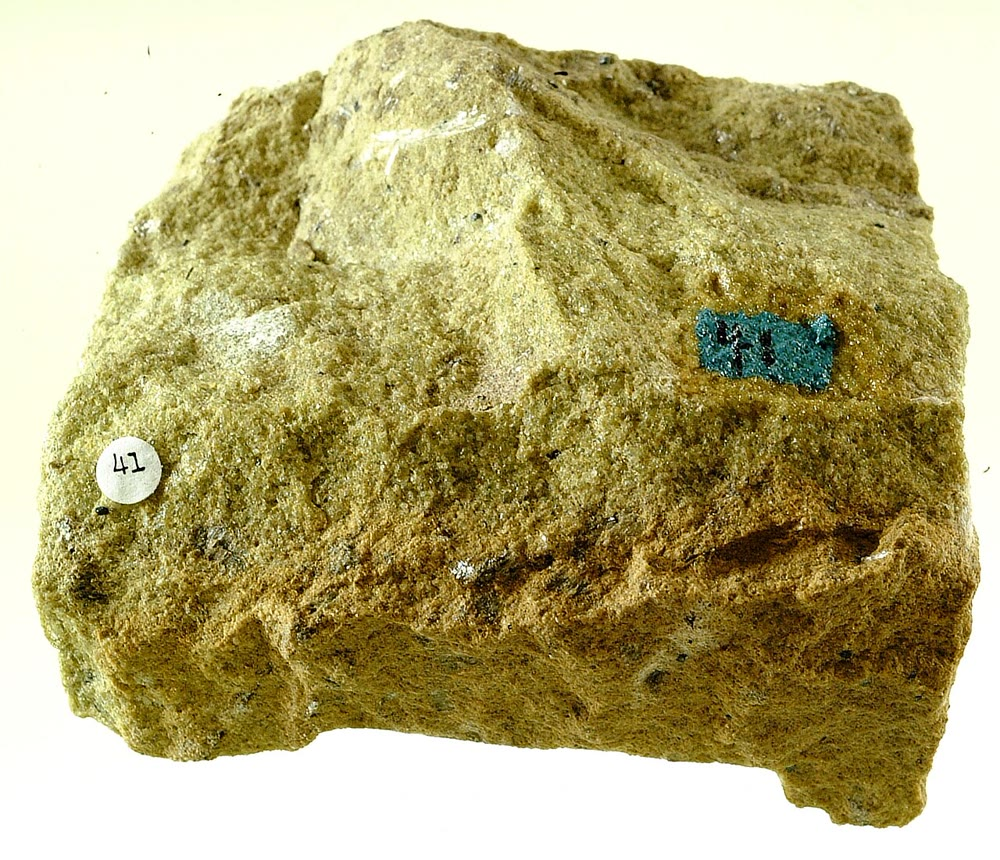
\includegraphics[width=\linewidth]{images/book4/b2-dunite.jpg}
\par\smallskip{\scriptsize Una \omterm{def:b2:mantle-melting:peridotites}{dunita}, casi toda de olivino, con pequeños granos negros
de cromita; la muestra mide \qty{8.5}{cm} (Mike Davis, CC0).}
\end{minipage}
\end{inthefield}
% ledger: casetta23:kimberlite, tulane:ocean-basins (Book 2), bgs:ultramafic

\section{Ejercicios}

\begin{exercise}[$\star$]\label{exo:b2:mantle-melting:1}
Nómbrese cada roca según sus proporciones de olivino, ortopiroxeno y clinopiroxeno
(por ciento): (a) 93, 5, 2; (b) 75, 25, 0; (c) 60, 27, 13; (d) 30, 45, 25. (e) Dese
el nombre del manto superior modelo (57, 28, 13 y \qty{2}{\percent} de espinela) tras
renormalizar sus tres silicatos al \qty{100}{\percent}.
\end{exercise}
% ledger: bgs:ultramafic, liang21:dmm-mode

\begin{exercise}[$\star$]\label{exo:b2:mantle-melting:2}
En el diagrama diópsido--anortita, se enfría un líquido con un \qty{60}{\percent} de anortita.
(a) ¿A qué temperatura empieza a cristalizar, y qué mineral
se forma? (b) ¿A qué temperatura aparece el segundo mineral, y cuál es entonces
la composición del líquido? (c) ¿Cuál es la composición del primer líquido cuando
se calienta una roca con un \qty{80}{\percent} de diópsido y un \qty{20}{\percent} de anortita,
y a qué temperatura aparece?
\end{exercise}
% ledger: bowen15:di-an

\begin{exercise}[$\star$]\label{exo:b2:mantle-melting:3}
(a) Calcúlese el gradiente adiabático $\alpha T/(\rho c_p)$ en kelvin por gigapascal
para $T_p = \qty{1350}{\celsius}$, $\alpha = \qty{4.0e-5}{K^{-1}}$, $\rho =
\qty{3300}{kg/m^3}$, $c_p = \qty{1000}{J/(kg.K)}$. (b) ¿Cuántos kilómetros de
manto forman un gigapascal ($g = \qty{9.81}{m/s^2}$)? Conviértase el gradiente a kelvin
por kilómetro y compárese con un gradiente geotérmico típico cerca de la superficie,
de unos \qty{30}{K/km}.
\end{exercise}
% ledger: katz03:thermo, earle:settings (Book 2)

\begin{exercise}[$\star$]\label{exo:b2:mantle-melting:4}
(a) Calcúlese el solidus seco de la \omterm{def:b2:mantle-melting:peridotites}{peridotita} a 0, 1, 2 y \qty{3}{GPa}. (b) ¿Cuántos
grados sube por gigapascal cerca de \qty{2}{GPa}? (c) Explíquese en una
frase por qué un manto a \qty{1400}{\celsius} a \qty{3}{GPa} es sólido, y el
mismo manto llevado a \qty{2}{GPa} sin intercambiar calor está parcialmente fundido.
\end{exercise}
% ledger: katz03:solidus

\begin{exercise}[$\star\star$]\label{exo:b2:mantle-melting:5}
Se enfría un líquido con un \qty{70}{\percent} de diópsido y un \qty{30}{\percent} de anortita.
(a) Estímese su temperatura de liquidus interpolando entre el liquidus con un
\qty{20}{\percent} de anortita (\qty{1350}{\celsius}) y con un \qty{40}{\percent}
(\qty{1277.5}{\celsius}). (b) ¿Qué mineral cristaliza primero? (c) ¿Qué fracción
másica del sistema ha cristalizado cuando el líquido alcanza el eutéctico?
(d) ¿Cuáles son las proporciones de diópsido y anortita en la roca final?
\end{exercise}
% ledger: bowen15:di-an

\begin{exercise}[$\star\star$]\label{exo:b2:mantle-melting:6}
(a) Calcúlese el porcentaje en masa de \ce{SiO2} en la forsterita \ce{Mg2SiO4} y en la
enstatita \ce{MgSiO3} ($M_{\ce{MgO}} = \qty{40.30}{g/mol}$, $M_{\ce{SiO2}} =
\qty{60.08}{g/mol}$). (b) Bowen y Andersen hallaron que el líquido peritéctico tenía un
\qty{97.5}{\percent} de \ce{MgSiO3} y un \qty{2.5}{\percent} de \ce{SiO2}: ¿cuál es su
contenido en sílice? (c) Úsese la regla de la palanca para calcular la fracción másica de forsterita
formada cuando la enstatita funde en el peritéctico, y compárese con su
\qty{5.5}{\percent}. (d) ¿Qué implica esto para el contenido en sílice de un fundido de
\omterm{def:b2:mantle-melting:peridotites}{peridotita} comparado con el de su ortopiroxeno?
\end{exercise}
% ledger: bowen14:mgo-sio2

\begin{exercise}[$\star\star$]\label{exo:b2:mantle-melting:7}
Con la adiabata $T = T_p + 20P$ y el solidus seco del texto, calcúlense la
presión y la profundidad ($\qty{30.9}{km}$ por gigapascal) a las que empieza la fusión
para (a) $T_p = \qty{1300}{\celsius}$ y (b) $T_p = \qty{1450}{\celsius}$. (c) ¿Cuántos
kilómetros por cada \qty{10}{\celsius} se profundiza el inicio cerca de
$T_p = \qty{1300}{\celsius}$? Úsese la \cref{prop:b2:mantle-melting:onset}.
\end{exercise}
% ledger: katz03:solidus

\begin{exercise}[$\star\star$]\label{exo:b2:mantle-melting:8}
A \qty{2.0}{GPa}, tómese una \omterm{def:b2:mantle-melting:fraction}{fracción de fundido} que crece linealmente desde el solidus seco hasta
el liquidus de la \omterm{def:b2:mantle-melting:peridotites}{lherzolita} $T_{\mathrm l} = 1475.0 + 80.0P - 3.2P^2$. Para $F = 0.10$:
(a) calcúlese la temperatura de la roca que se funde; (b) calcúlense $(\partial
T/\partial P)_F$ y $(\partial T/\partial F)_P$; (c) calcúlese la productividad con
$c_p = \qty{1000}{J/(kg.K)}$, $\alpha/\rho = \qty{1.21e-8}{m^3/(kg.K)}$ y
$\Delta S = \qty{300}{J/(kg.K)}$. (d) ¿Cuánto valdría sin calor latente?
\end{exercise}
% ledger: katz03:solidus, katz03:melting, katz03:thermo

\begin{exercise}[$\star\star$]\label{exo:b2:mantle-melting:9}
(a) ¿Cuánto rebajan el solidus un 1, un 5 y un \qty{13}{\percent} de agua disuelta en el
fundido? (b) ¿Cuál es el solidus saturado en agua a \qty{1}{GPa}? (c) Un manto
contiene \qty{125}{ppm} de agua en masa, y el coeficiente de reparto del agua entre
minerales y fundido es 0.01. En la primerísima fusión, el fundido contiene $X =
X_{\text{global}}/D$: calcúlese, y el descenso del solidus que causa.
\end{exercise}
% ledger: katz03:water

\begin{exercise}[$\star\star\star$]\label{exo:b2:mantle-melting:10}
(a) En la \cref{prop:b2:mantle-melting:triangle}, compruébese que el manto que entra por la
base del triángulo cada año es igual al manto que sale por sus lados. ¿Por qué
deben estar los lados a \ang{45} para un manto que sube a $U$ y sale a $U$?
(b) Demuéstrese que, con una productividad constante $\Pi$ por gigapascal, $h_c = \Pi\,\rho
g\,z_0^2/2$ (con $P_0 = \rho g z_0$), de modo que la corteza crece como el cuadrado de la
profundidad del inicio. (c) Una dorsal se expande a una velocidad total de \qty{50}{mm/yr} y
produce \qty{7.1}{km} de corteza: ¿qué volumen de corteza produce cada kilómetro de dorsal
al año, y qué volumen de manto funde si la \omterm{def:b2:mantle-melting:fraction}{fracción de fundido} media es del
\qty{12}{\percent}?
\end{exercise}

\begin{exercise}[$\star\star\star$]\label{exo:b2:mantle-melting:11}
En el sistema ternario de la figura esquemática, el líquido $X$ tiene un
\qty{60}{\percent} de A, un \qty{20}{\percent} de B y un \qty{20}{\percent} de C; el
eutéctico binario $e_{AB}$ está en A 40, B 60 (por ciento), y el \omterm{def:b2:mantle-melting:ternary}{eutéctico ternario} E en
A 25, B 30, C 45. (a) Escríbase la composición del líquido cuando ha cristalizado una fracción másica $t$
de A puro, y demuéstrese que la razón de B a C se mantiene en 1. (b) La
cotéctica de $e_{AB}$ a E es la línea de los puntos $e_{AB} + s(E - e_{AB})$: hállese
dónde la encuentra el líquido, y la fracción de A cristalizada hasta entonces. (c) Cuando
el líquido alcanza E, ¿qué fracción del sistema sigue siendo líquida? (C no entra en ningún
cristal antes de E.) (d) ¿Cuánto A y cuánto B han cristalizado hasta entonces?
\end{exercise}

\begin{exercise}[$\star\star\star$]\label{exo:b2:mantle-melting:12}
El contenido en agua de un fundido saturado es $X_{\mathrm{sat}} = 12P^{0.6} + P$
(por ciento, con $P$ en gigapascales). (a) Calcúlense a 1 y a \qty{2}{GPa}, el descenso del solidus
que produce y el solidus saturado en agua a ambas presiones. (b) ¿Por qué
el solidus saturado apenas cambia entre 1 y \qty{2}{GPa} mientras que el seco
sube más de \qty{100}{\celsius}? (c) En una cuña del manto a \qty{2}{GPa} y
\qty{1100}{\celsius}, ¿cuánta agua debe contener el fundido para que la roca se funda?
\end{exercise}
% ledger: katz03:water, katz03:solidus

\section{Problema: Bajo la dorsal}

\begin{problem}[{Problema de fin de semana --- de la adiabata del manto al espesor de
la corteza oceánica, y de vuelta a la temperatura del manto}]
\label{pb:b2:mantle-melting:1}
El manto sube bajo una dorsal a lo largo de la adiabata y se funde. Datos: coeficiente de
dilatación térmica $\alpha = \qty{4.0e-5}{K^{-1}}$; densidad $\rho = \qty{3300}{kg/m^3}$;
calor específico $c_p = \qty{1000}{J/(kg.K)}$; entropía de fusión $\Delta S =
\qty{300}{J/(kg.K)}$; $g = \qty{9.81}{m/s^2}$; solidus seco $T_{\mathrm s} =
1085.7 + 132.9P - 5.1P^2$ y liquidus de la \omterm{def:b2:mantle-melting:peridotites}{lherzolita} $T_{\mathrm l} = 1475.0 +
80.0P - 3.2P^2$ (\unit{\celsius}, con $P$ en \unit{GPa}); productividad media del
modelo de fusión ajustado, $\Pi = \qty{9}{\percent}$ por gigapascal; coeficiente de reacción del
clinopiroxeno cerca de la superficie, 0.50; corteza observada, \qty[uncertainty-mode=separate]{7.1 \pm 0.8}{km}
en las dorsales normales y \qty{20}{km} sobre el núcleo de la pluma de Islandia. Tómense el manto
y la corteza de la misma densidad.

\noindent\textbf{Parte I --- Dónde empieza la fusión.}
\begin{enumerate}
\item Conviértase $T_p = \qty{1350}{\celsius}$ a kelvin.
\item Calcúlese el gradiente adiabático $\alpha T_p/(\rho c_p)$ en kelvin por
gigapascal, y redondéese a la decena más próxima.
\item ¿Cuántos kilómetros de manto forman un gigapascal? Dese el gradiente en
kelvin por kilómetro.
\item Con la adiabata $T = 1350 + 20P$, escríbase la ecuación de segundo grado de la presión de inicio
$P_0$ y resuélvase.
\item Dense la profundidad y la temperatura a las que empieza la fusión.
\item Compruébese que el solidus en $P_0$ da la misma temperatura.
\end{enumerate}

\noindent\textbf{Parte II --- Cuánto fundido.}
\begin{enumerate}[resume]
\item A \qty{1.5}{GPa}, calcúlense el solidus, el liquidus de la \omterm{def:b2:mantle-melting:peridotites}{lherzolita} y su
diferencia.
\item Con una \omterm{def:b2:mantle-melting:fraction}{fracción de fundido} que crece linealmente entre ambos, dese la temperatura de
la roca para $F = 0.10$, en grados Celsius y en kelvin.
\item Calcúlense allí $(\partial T/\partial P)_F$ y $(\partial T/\partial F)_P$.
\item Calcúlese la productividad de la \cref{prop:b2:mantle-melting:productivity}, en
tanto por ciento por gigapascal.
\item El modelo ajustado da de media $\Pi = \qty{9}{\percent}$ por gigapascal.
¿Por qué es menor? Con $\Pi$, ¿qué \omterm{def:b2:mantle-melting:fraction}{fracción de fundido} $F_{\max}$ se alcanza en la
superficie?
\item El manto modelo contiene un \qty{13}{\percent} de clinopiroxeno. ¿Con qué \omterm{def:b2:mantle-melting:fraction}{fracción
de fundido} se agota cerca de la superficie? ¿Es el residuo bajo el eje una
\omterm{def:b2:mantle-melting:peridotites}{lherzolita} o una \omterm{def:b2:mantle-melting:peridotites}{harzburgita}?
\end{enumerate}

\noindent\textbf{Parte III --- La corteza.}
\begin{enumerate}[resume]
\item Úsese la \cref{prop:b2:mantle-melting:triangle} con $H = z_0$ para calcular el
espesor de la corteza.
\item ¿Cuál es la \omterm{def:b2:mantle-melting:fraction}{fracción de fundido} media del fundido agregado?
\item Compárese con el espesor observado.
\item El modelo completo de la figura da \qty{9.0}{km}. ¿Por qué es más delgado que
la estimación obtenida?
\item Demuéstrese que $h_c = k P_0^2$ y calcúlese $k$ en kilómetros por gigapascal
al cuadrado.
\end{enumerate}

\noindent\textbf{Parte IV --- La temperatura del manto.}
\begin{enumerate}[resume]
\item Calcúlese la presión de inicio $P_0$ que produce \qty{7.1}{km} de corteza.
\item Dese la profundidad correspondiente del inicio.
\item Con la adiabata $T = T_p + 20P$, calcúlese la temperatura potencial que
sitúa el inicio a esa presión.
\item Rehágase el cálculo para 6.3 y \qty{7.9}{km}: ¿qué intervalo de $T_p$ permite la
dispersión de la corteza?
\item La corteza tiene \qty{20}{km} de espesor sobre el núcleo de la pluma de Islandia. Calcúlese
allí la temperatura potencial, y su exceso sobre la de la pregunta~20.
\item Las lavas de las islas oceánicas sugieren plumas de 200 a \qty{300}{\celsius} más calientes que
el manto circundante. Propóngase por qué la corteza da un exceso menor.
\item ¿En qué porcentaje se engrosa la corteza para un manto \qty{10}{\celsius}
más caliente, cerca de la dorsal normal?
\item Las dorsales muy lentas producen una corteza más delgada. Explíquese por qué con el triángulo.
\item Dese la \omterm{def:b2:mantle-melting:tp}{temperatura potencial del manto} bajo una dorsal normal que da el
espesor de la corteza, el número clave de este problema, y compárese
con los \qty{1350}{\celsius} de la física de minerales y con el intervalo de 1280 a
\qty{1400}{\celsius} de las lavas.
\end{enumerate}
\end{problem}
% ledger: katz03:solidus, katz03:melting, katz03:thermo, white:crust (Book 3), herzberg:tp (Book 3), katsura:adiabat (Book 3)
